\chapter{Конструкторская часть}

В данном разделе приведены схемы алгоритмов сортировок - бусинами, пирамидальная, Шелла, приведено описанию используемых типов данных.

\section{Требования к программному обеспечению}

К программе предъявлены ряд функциональных требований: входные данные --- массив и размер массива, выходные данные --- отсортированный массив.

К программе предъявлены ряд требований:

\begin{itemize}[label=---]
	\item должна иметь интерфейс для выбора действий;
	\item должна динамически выделять память под массив данных;
	\item должна замерять процессорное время работы реализации алгоритмов.
\end{itemize}

\section{Разработка алгоритмов}

На вход алгоритмов подаются указатель на массив $array$ и размер массива $n$ - целое положительное число.

На рисунках \ref{fig:Shell} -- \ref{fig:bead} представлены схемы алгоритмов сортировок, а именно сортировка Шелла, пирамидальная сортировка и сортировка бусинами.

\begin{figure}[h]
	\centering
	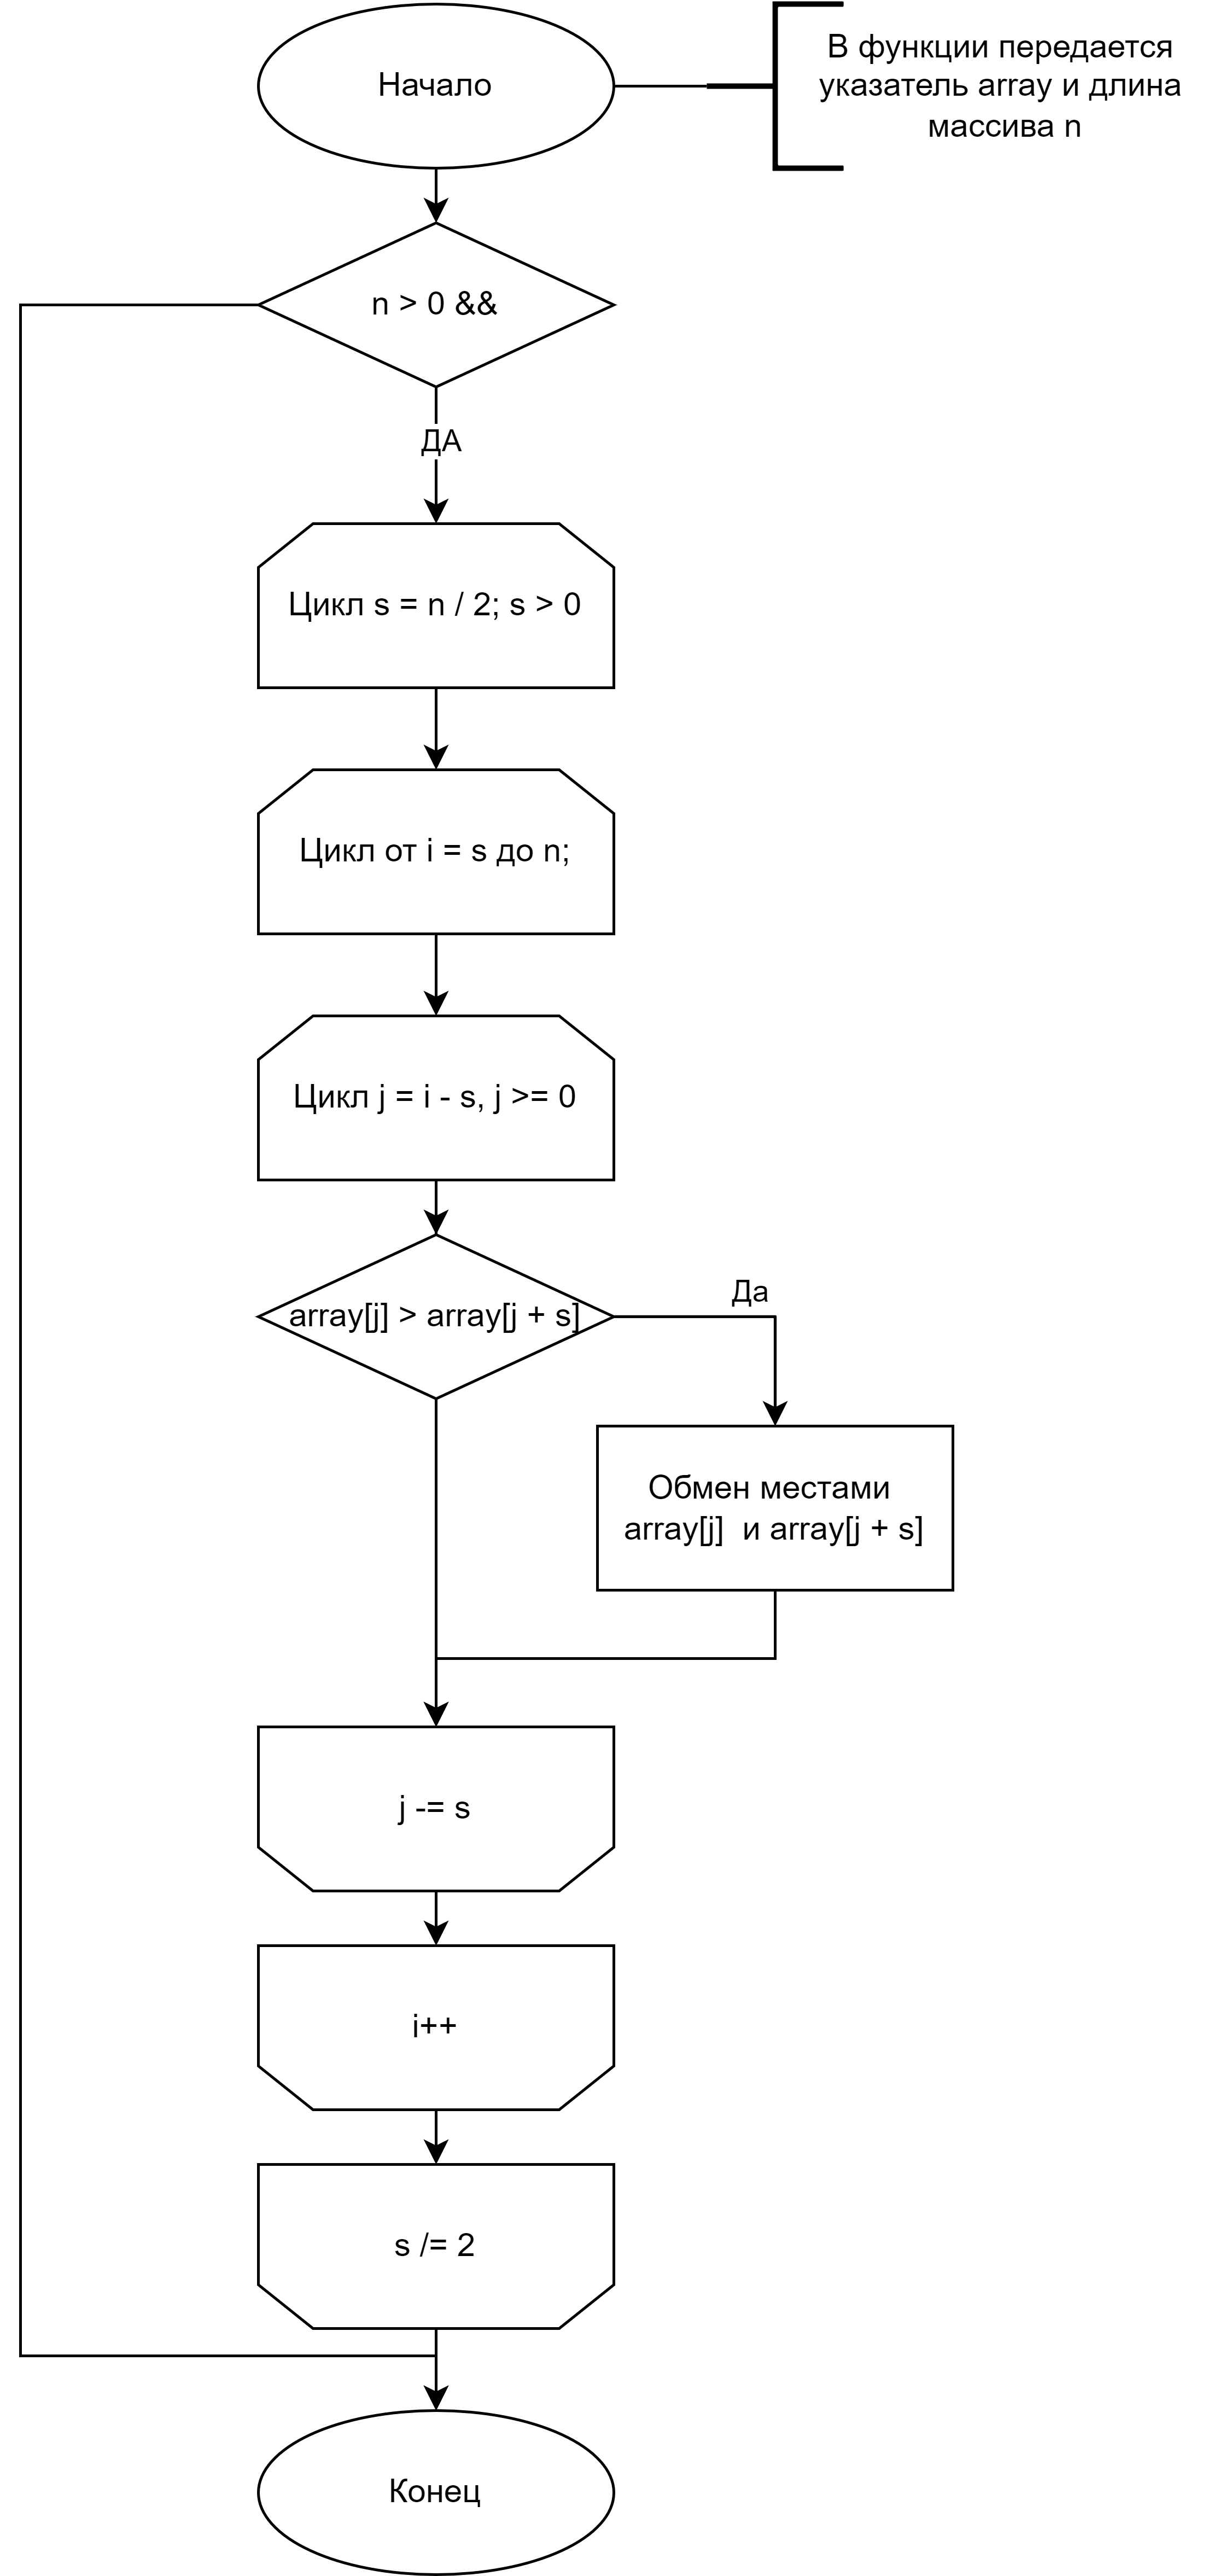
\includegraphics[height=0.8\textheight]{img/shell.png}
	\caption{Схема алгоритма сортировки методом Шелла}
	\label{fig:Shell}
\end{figure}

\clearpage

\begin{figure}[h]
	\centering
	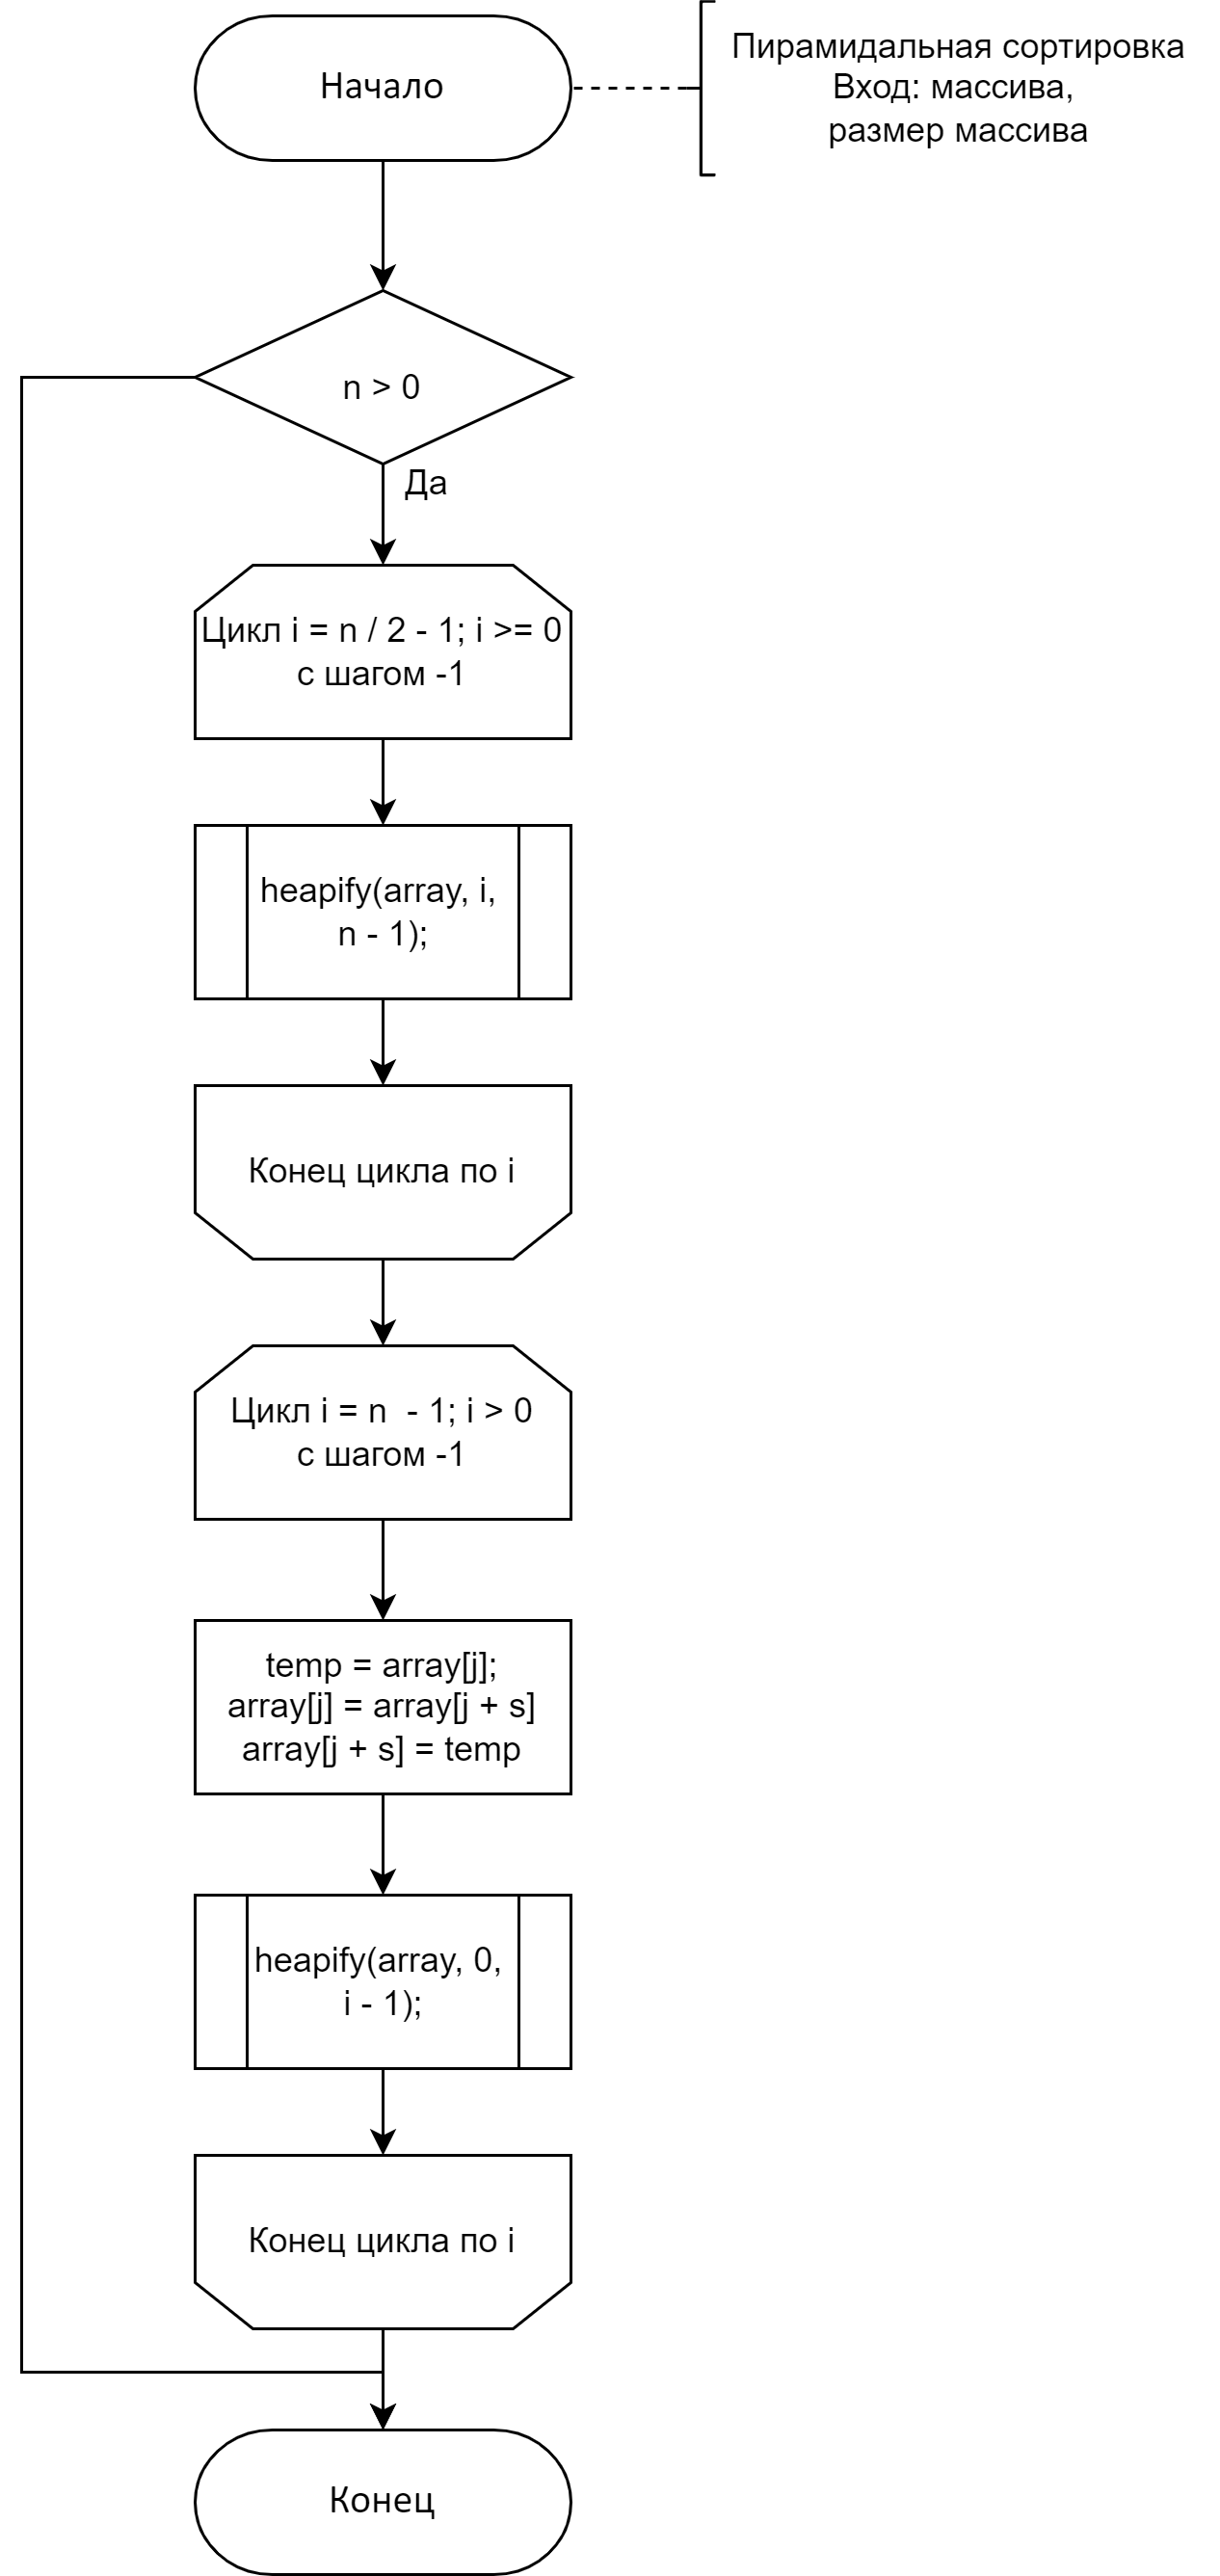
\includegraphics[height=0.8\textheight]{img/heap_1.png}
	\caption{Схема алгоритма пирамидальной сортировки}
	\label{fig:heap_1}
\end{figure}

\clearpage

\begin{figure}[h]
	\centering
	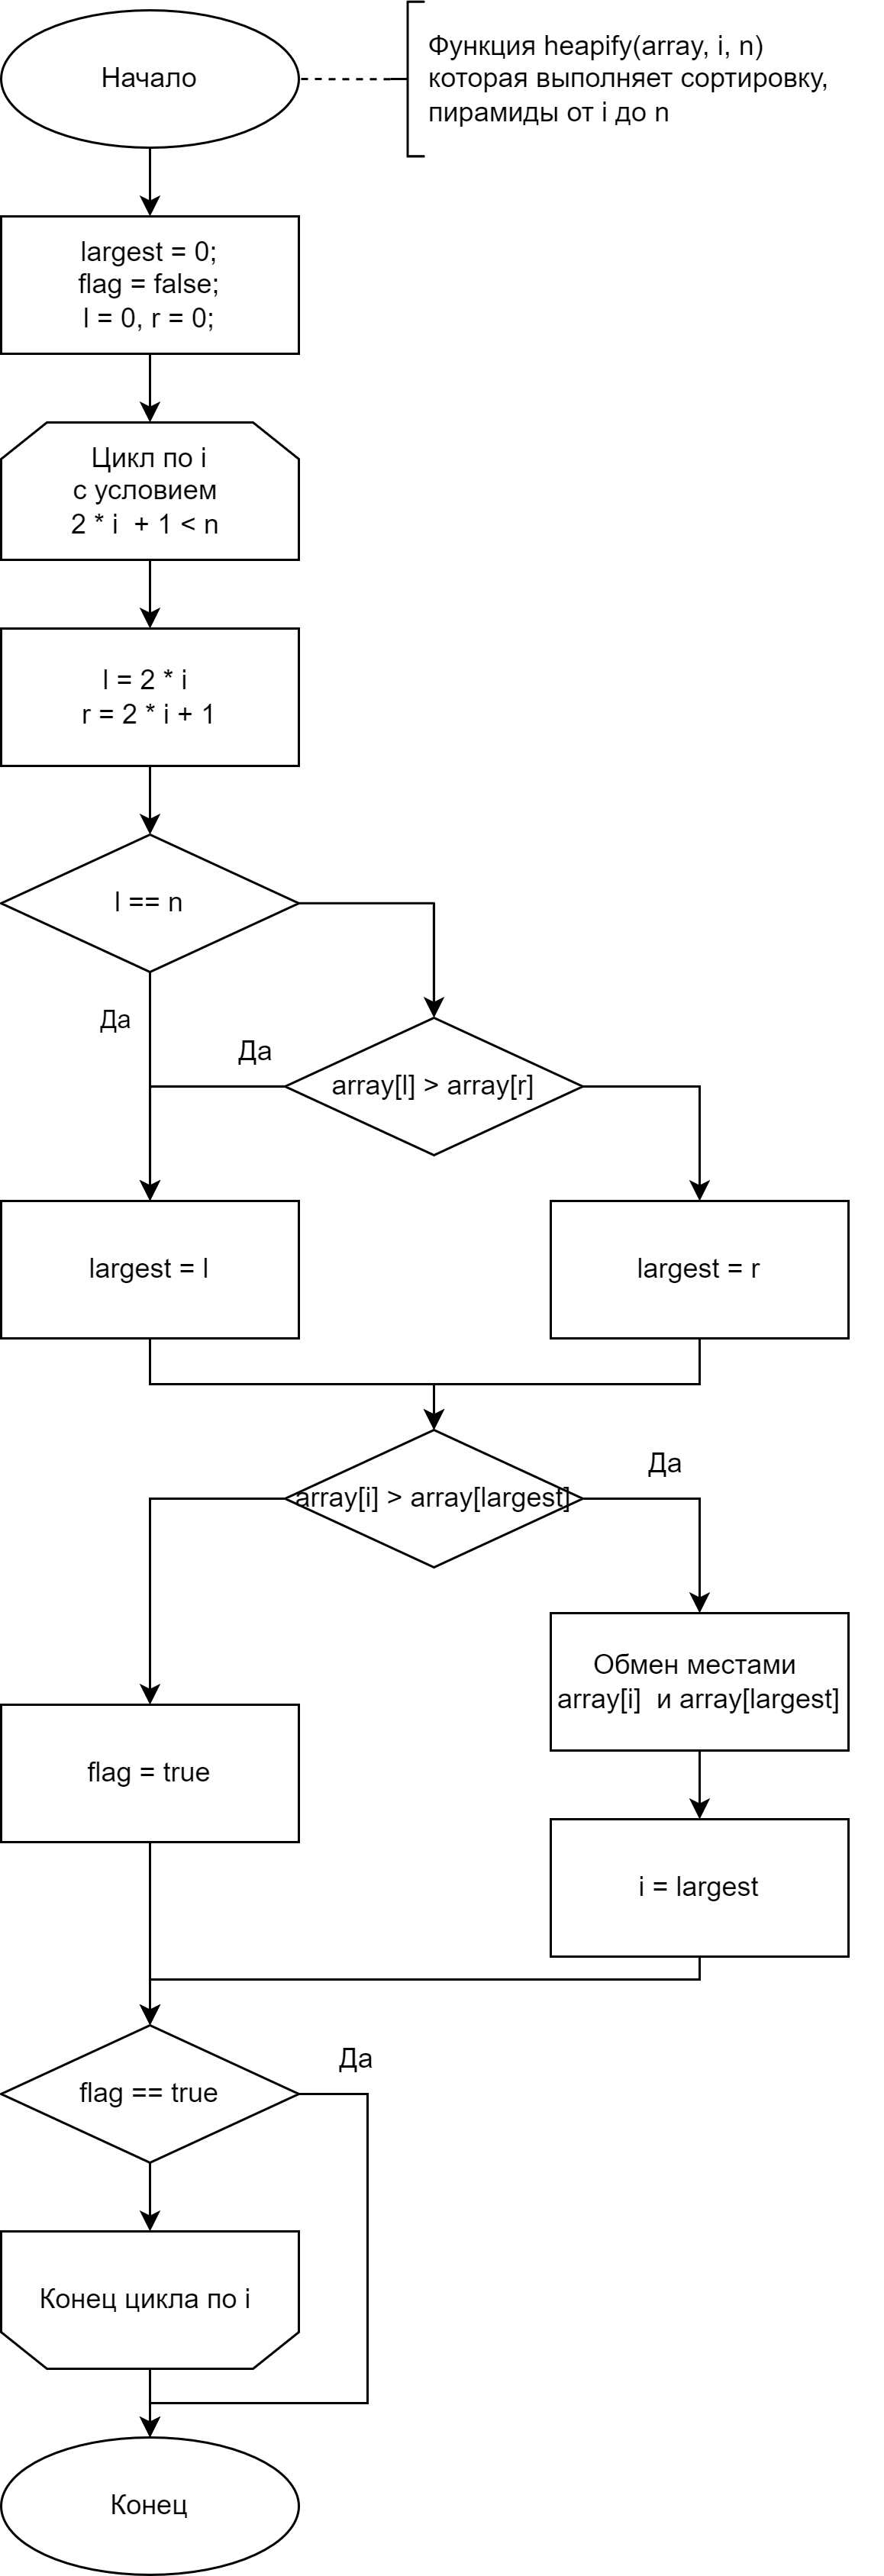
\includegraphics[height=0.8\textheight]{img/heap_2.png}
	\caption{Схема алгоритма функции heapify() для пирамидальной сортировки}
	\label{fig:heap_2}
\end{figure}

\clearpage

\begin{figure}[h]
	\centering
	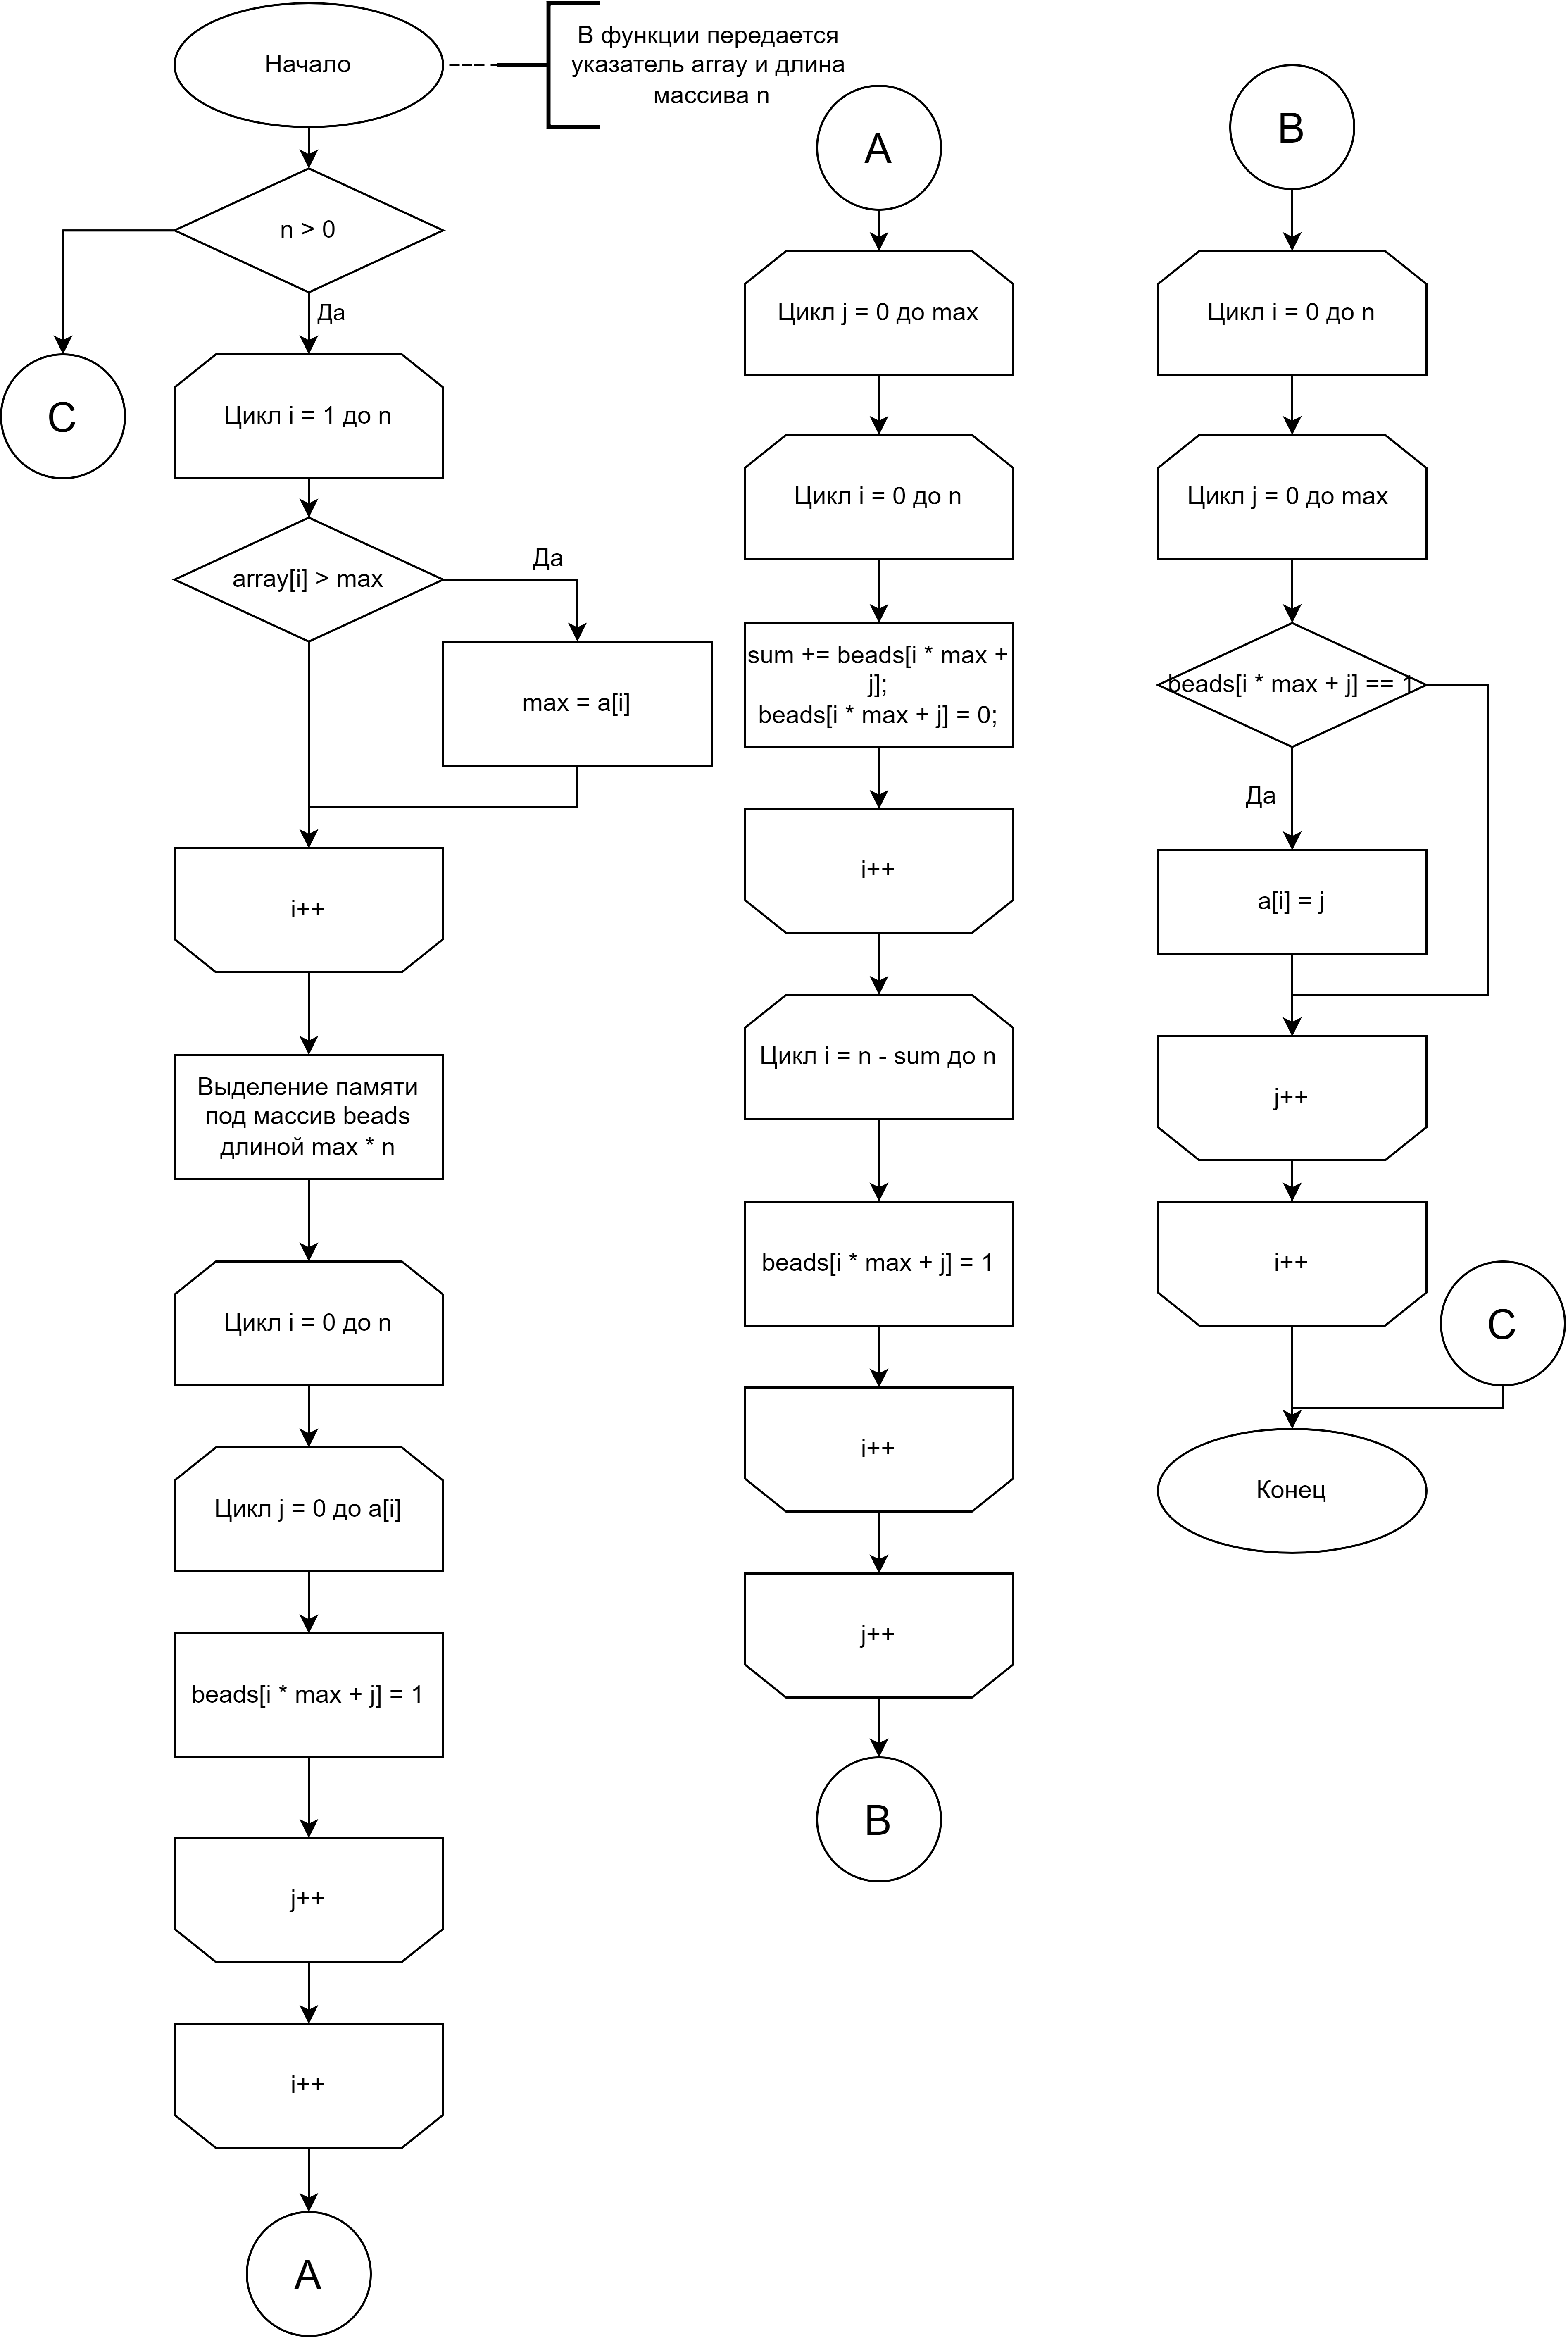
\includegraphics[height=0.8\textheight]{img/bead.png}
	\caption{Схема алгоритма сортировки бусинами}
	\label{fig:bead}
\end{figure}

\clearpage

\section{Описание используемых типов данных}

При реализации алгоритмов будут использованы следующие структуры данных:

\begin{itemize}[label=---]
	\item указатель на массив типа $int *$;
	\item массив типа $int$;
	\item длина массива - целое число типа $size\_t$
\end{itemize}

\section{Модель вычислений для проведения \newline оценки трудоемкости}

Введем модель вычислений, которая потребуется для определения трудоемкости каждого отдельного взятого алгоритма сортировки.
\begin{enumerate}[label={\arabic*)}]
	\item Трудоемкость базовых операций имеет:
	\begin{itemize}[label=---]
		\item равную 1:
		\begin{equation}
			\label{for:operations_1}
			\begin{gathered}
				+, -, =, +=, -=, ==, !=, <, >, <=, >=, [], ++, {-}-,\\
				\&\&, >>, <<, ||, \&, |
			\end{gathered}
		\end{equation}
		\item равную 2:
		\begin{equation}
			\label{for:operations_2}
			*, /, \%, *=, /=, \%=
		\end{equation}
	\end{itemize}
	\item Трудоемкость условного оператора:
	\begin{equation}
		\label{for:if}
		f_{if} = f_{\text{условия}} + 
		\begin{cases}
			min(f_1, f_2), & \text{лучший случай}\\
			max(f_1, f_2), & \text{худший случай}
		\end{cases}
	\end{equation}
	\item Трудоемкость цикла:
	\begin{equation}
		\label{for:for}
		\begin{gathered}
			f_{for} = f_{\text{инициализация}} + f_{\text{сравнения}} + M_{\text{итераций}} \cdot (f_{\text{тело}} +\\+ f_{\text{инкремент}}
			+ f_{\text{сравнения}})
		\end{gathered}
	\end{equation}
	\item Трудоемкость передачи параметра в функции и возврат из функции равен 0.
\end{enumerate}

\section{Трудоемкость алгоритмов сортировки}

\subsection{Алгоритм сортировки Шелла}

Трудоемкость в лучшем случае при отсортированном массиве, когда ничего не обменивается, но все же данные рассматриваются. Выведена \newline формуле (\ref{сomplexity:shell_best}).
\begin{equation}
	\label{сomplexity:shell_best}
	\begin{gathered}
		f_{best} = 3 + 4 + \frac{N}{4} \cdot (3 + 2 + log(N) \cdot (2 + 4 + 4)) = \\
		= 7 + \frac{5N}{4} + \frac{5N \cdot log(N)}{2} = O(N \cdot log(N))
	\end{gathered}
\end{equation}

Трудоемкость в худшем случае при отсортированном массиве в обратном порядке. Выведена формуле (\ref{сomplexity:shell_worst}).
\begin{equation}
	\label{сomplexity:shell_worst}
	\begin{gathered}
		f_{worst} = 7 + \frac{N}{4} \cdot (5 + log(N) \cdot (10 + log(N) \cdot (6 + 4))) =\\
		= 7 + \frac{5N}{4} + \frac{5N \cdot log(N)}{2} + \frac{5N \cdot log^2(N)}{2} = O(N \cdot log^2(N))
	\end{gathered}
\end{equation}

\clearpage

\subsection{Алгоритм пирамидальной сортировки}

Трудоемкость в лучшем случае при отсортированном массиве. Выведена формуле (\ref{сomplexity:heap_best_t}).
\begin{equation}
	\label{сomplexity:heap_best_t}
	\begin{gathered}
		f_{best} = 3 + 4 + \frac{N}{2} \cdot (2 + 1 + f_{heapify\_best}) + \\
		+ 3 + (N - 1)(2 + 2 + f_{swap} + 1 + f_{heapify\_best})
	\end{gathered}
\end{equation}

Трудоемкость в худшем случае при отсортированном массиве в обратном порядке. Выведена в формуле (\ref{сomplexity:heap_worst_t}).

\begin{equation}
	\label{сomplexity:heap_worst_t}
	\begin{gathered}
		f_{worst} = 3 + 4 + \frac{N}{2} \cdot (2 + 1 + f_{heapify\_worst}) + \\
		+ 3 + (N - 1)(2 + 2 + f_{swap} + 1 + f_{heapify\_worst})
	\end{gathered}
\end{equation}

Трудоемкость перестановки элементов будет равна, формула (\ref{сomplexity:swap})
\begin{equation}
	\label{сomplexity:swap}
	f_{swap} = 1 + 1 + 1 = 3
\end{equation}

Трудоемкость части программы сортировки пирамиды является функция heapify, формула (\ref{сomplexity:heapify}).

\begin{equation}
	\label{сomplexity:heapify}
	f_{heapify} = 5 + log N \cdot (5 + 3 + 4 + 1 + 
	\begin{cases}
		1, \\
		3 + \begin{cases}
			1, \\
			1,
		\end{cases},
	\end{cases} + 3 +
	\begin{cases}
		1, \\
		4,
	\end{cases})
\end{equation}

Исходя из формулы (\ref{сomplexity:heapify}) были выведены лучший (\ref{сomplexity:heapify_best}) и худший (\ref{сomplexity:heapify_worst}) случаи функции heapify:

\begin{equation}
	\label{сomplexity:heapify_best}
	f_{heapify\_best} = 5 + log N \cdot (5 + 3 + 4 + 2 + 4) = 5 + 17 \cdot log N = O(log N) 
\end{equation}

\begin{equation}
	\label{сomplexity:heapify_worst}
	f_{heapify\_worst} = 5 + log N \cdot (5 + 3 + 4 + 5 + 7) = 5 + 24 \cdot log N = O(log N) 
\end{equation}

Исходя из выведенных выше, то лучший и худший случаи будут равны: 

\begin{equation}
	\label{сomplexity:heap_best_p}
	\begin{gathered}
		f_{best} = 7 + \frac{N}{2} \cdot (3 + 5 + 17 \cdot log N) + 3 + (N - 1) \cdot (5 + 3 + \\ 
		+ 5 + 17 \cdot log N) = 23N + 27N \cdot log N - 13 \cdot log N - 3 =\\
		= O(N \cdot log N)
	\end{gathered}
\end{equation}

\begin{equation}
	\label{сomplexity:heap_worst_p}
	\begin{gathered}
		f_{worst} = 7 + \frac{N}{2} \cdot (3 + 5 + 24 \cdot log N) + 3 + (N - 1) \cdot (5 + 3 + \\ 
		+ 5 + 24 \cdot log N) = 23N + 36N \cdot log N - 24 \cdot log N - 3 =\\
		= O(N \cdot log N)
	\end{gathered}
\end{equation}

Таким образов из выведенных результатов в формулах (\ref{сomplexity:heap_best_p}) и (\ref{сomplexity:heap_worst_p}) можно понять, что лучший и худший случай имеют трудоемкость $O(N \cdot log N)$.

\subsection{Алгоритм сортировки бусинами}

Трудоемкость в лучшем случае при отсортированном массиве и худшем случае при неотсортированном массиве в обратном порядке.Выведена формуле \ref{сomplexity:bead}.
\begin{equation}
	\label{сomplexity:bead}
	\begin{gathered}
		f_{best} = 3 + 4 + (N - 1) \cdot (2 + 2 + 
		\begin{cases}
			0, \\
			2,
		\end{cases}) 
		+ 1 + 2 + \\
		+ N \cdot (2 + 3 + L \cdot (3 + 5)) + 2 + M \cdot (2 + 3 + N \cdot (2 + 5 + 5) + \\
		+3 + (N - L) \cdot (2 + 5)) + 2 + N \cdot (2 + 8 + 8M) = \\
		= S + 19NM + 11N + 8M + 18 = O(S)
	\end{gathered}
\end{equation}

В формуле (\ref{сomplexity:bead}) значения $S$ или $NL$ --- сумма всех элементов в изначальном массиве, $L$ --- значение каждого элемента в массиве,  M --- максимальное значение из элементов в массиве.

Исходя из результата формулы (\ref{сomplexity:bead}) можно понять, что лучшим случаем для сортировки будет случай если все значения массива будут соответствовать минимальному значению, а худшим случаем если значение массива будут большие значения. 

\section*{Вывод}

В данном разделе на основе теоретических данных были построены схемы
требуемых алгоритмов, выбраны используемые типы данных. Для каждого алгоритма сортировки были выведены трудоемкости худшего и лучшего случаев.